\documentclass[conference]{IEEEtran}
\IEEEoverridecommandlockouts
% The preceding line is only needed to identify funding in the first footnote. If that is unneeded, please comment it out.
\usepackage{cite}
\usepackage{amsmath,amssymb,amsfonts}
\usepackage{algorithmic}
\usepackage{graphicx}
\usepackage{textcomp}
\usepackage{xcolor}
\usepackage{float}
\usepackage{url}
\def\BibTeX{{\rm B\kern-.05em{\sc i\kern-.025em b}\kern-.08em
    T\kern-.1667em\lower.7ex\hbox{E}\kern-.125emX}}
\begin{document}

\title{HOMEWOEK 2}

\author{\IEEEauthorblockN{Runlin Hou}
\IEEEauthorblockA{\textit{ECE, School Of Graduate Studies} \\
\textit{Rutgers University}\\
hourunlinxa@gmail.com}
}

\maketitle

\subsection*{Question 1}
We know that insertion sort would face the worst case when the sequence is 
exactly reverse order. And for the usual case, it shows a better performence
when the sequence are almost sorted. And shell sort is actually taking some 
former step to sort part of the sequence first. Then it would be much more 
effective when doing the insertoin sort.

To test the performance, I use some reverse sequence lengnth from 10 to 10240.
As we can see on the picture, the comparision made by insertion sort is way more 
than shell sort, which leads to the increase of the time.

\begin{figure}[H]
    \centerline{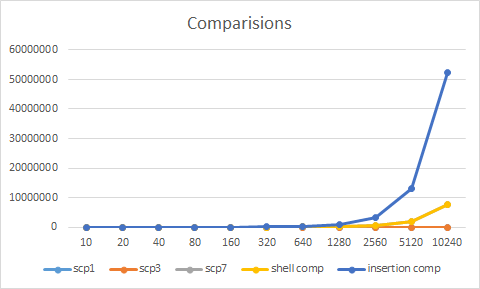
\includegraphics[scale=0.05]{Pic/pic1.png}}
\end{figure}

\begin{figure}[H]
    \centerline{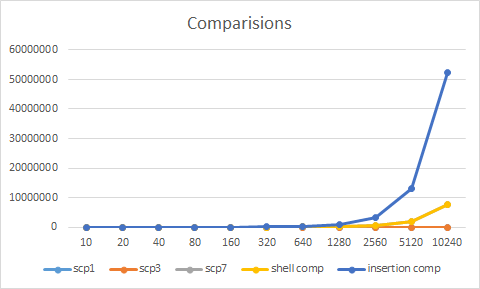
\includegraphics[scale=0.05]{Pic/pic1.png}}
\end{figure}

\end{document}